%
% software.tex
%
%
% \author Christian Galvez <chant4@vt.edu>
%
% \institution Virginia Polytechnic Institute of Technology (VT)
%
% \version 1.0.0
%
% \date 2025/09/26
%

\chapter{Software} \label{ch:software}

The app provides many key features of interest, particularly for realtors and land-owners looking to see zoning specifics for their county of interest. This chapter will delve into the specifics of what exactly this app is capable of.

\begin{figure}[H]
    \centering
    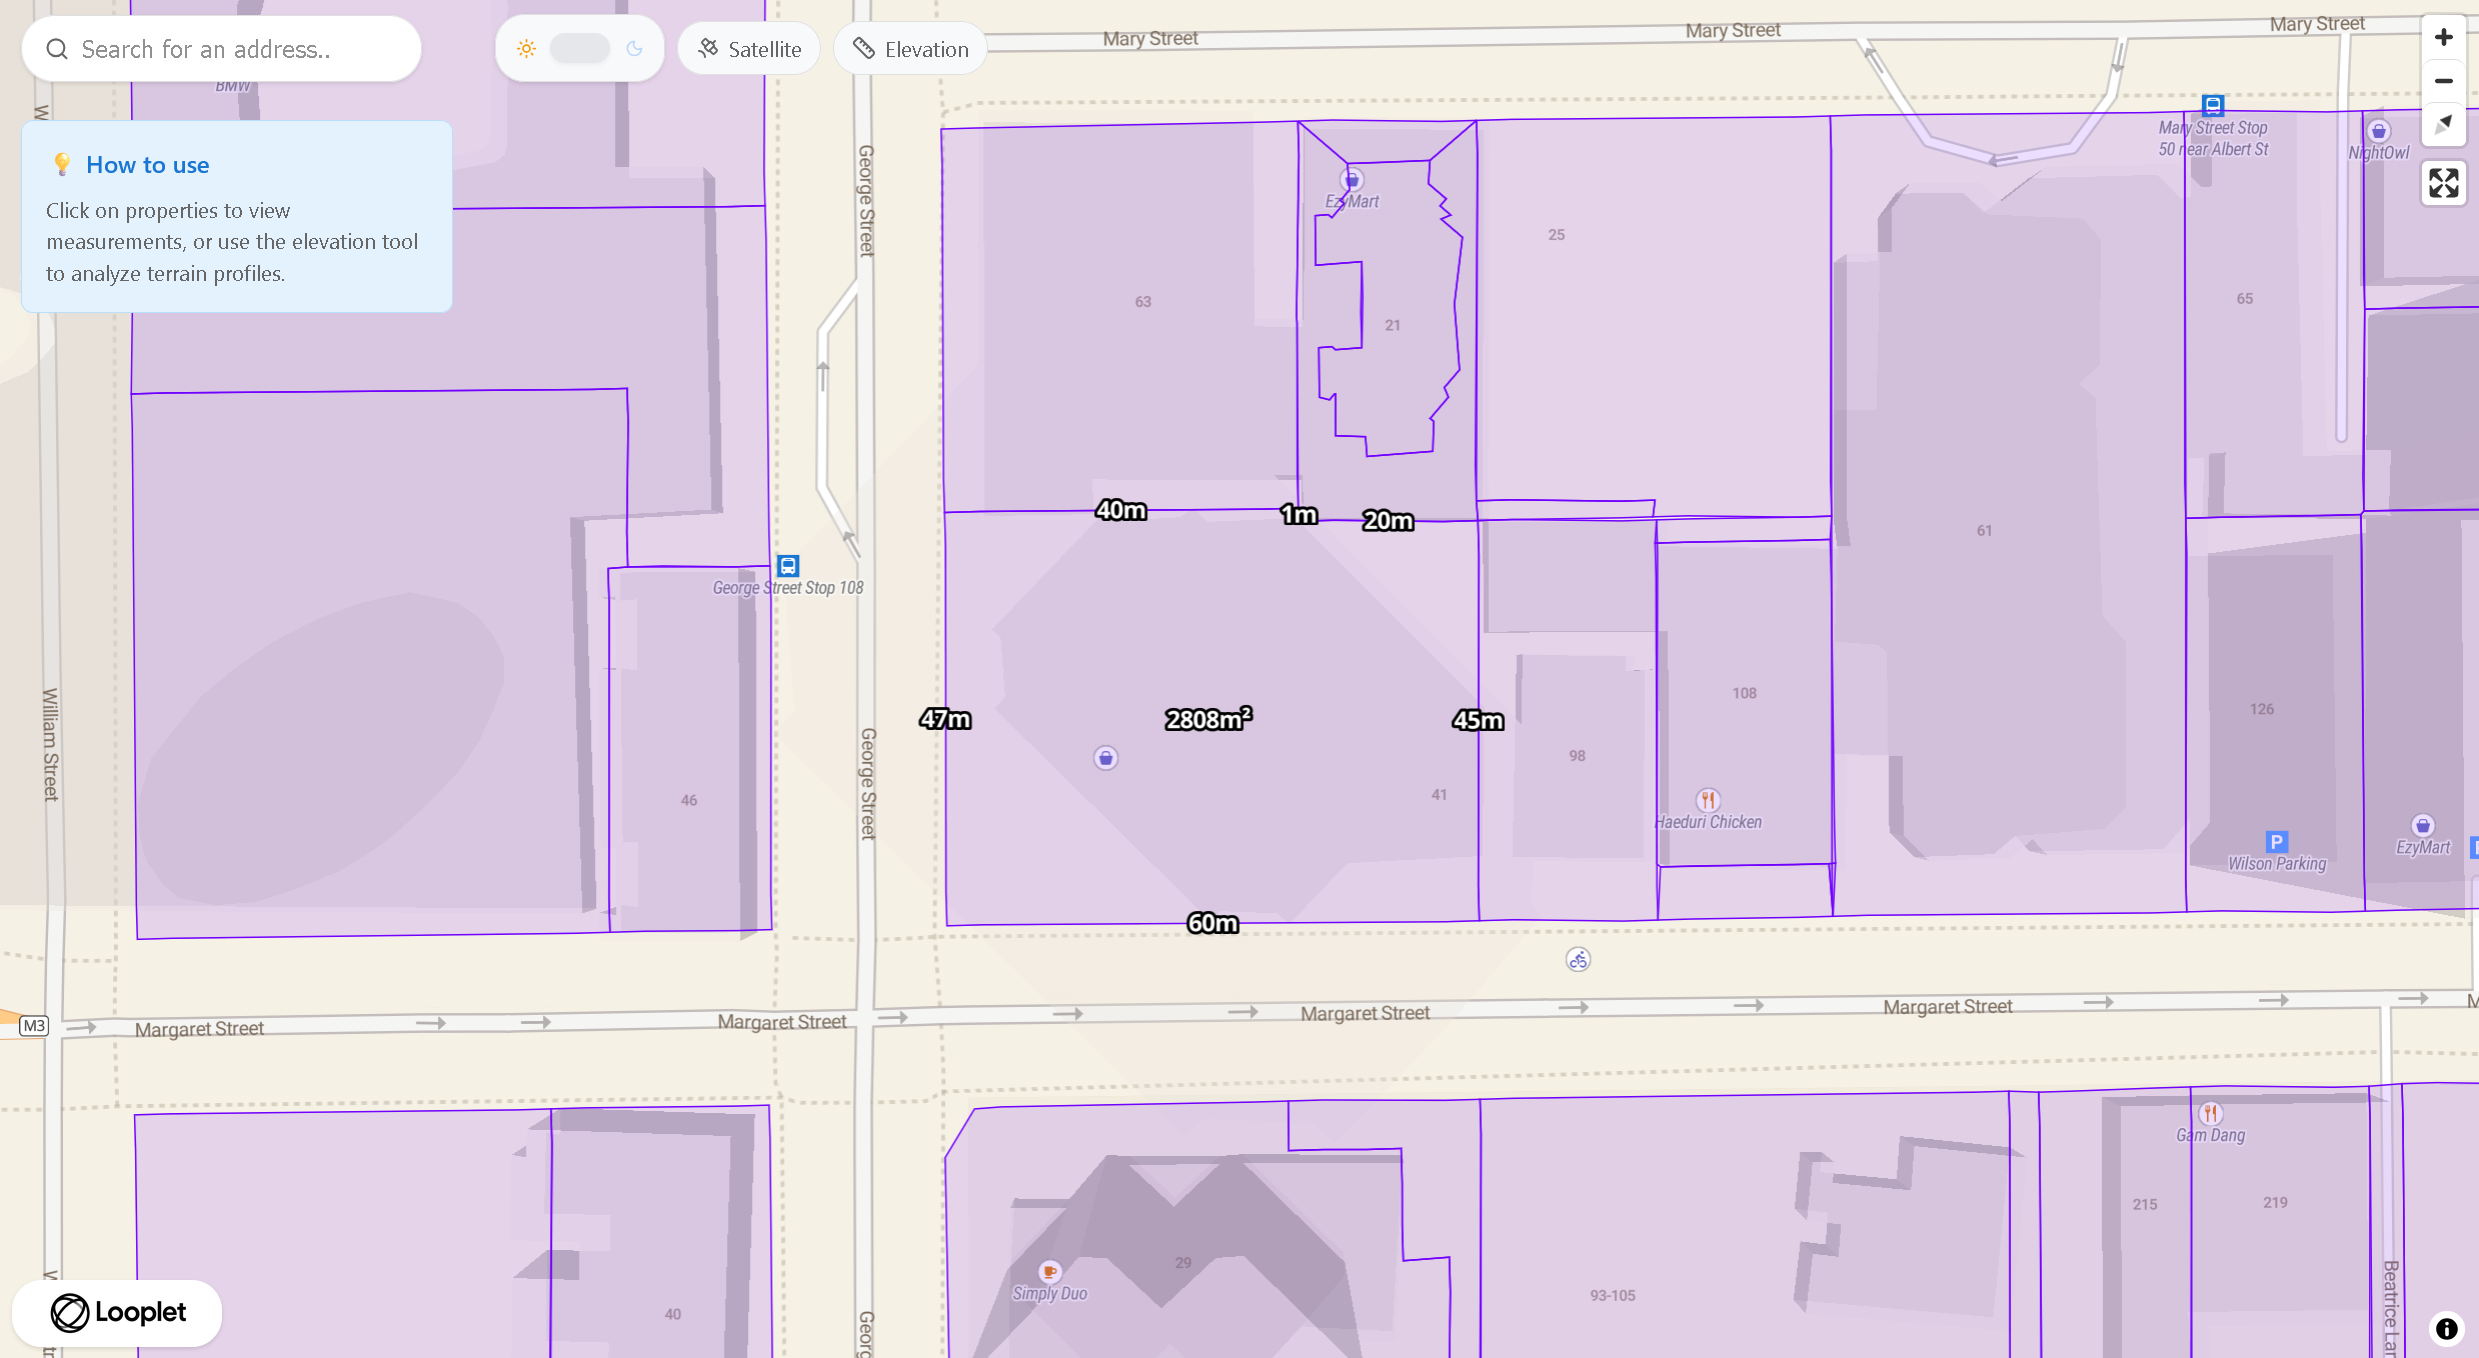
\includegraphics[scale=0.15]{figures/top_down_view.png}
    \caption{Top-down view}
\end{figure}

This is the standard view a user will see upon first opening the app. 

\begin{figure}[H]
    \centering
    \includegraphics[scale=0.15]{figures/satellite_view.png}
    \caption{Satellite view}
\end{figure}

Users can see a satellite.

\begin{figure}[H]
    \centering
    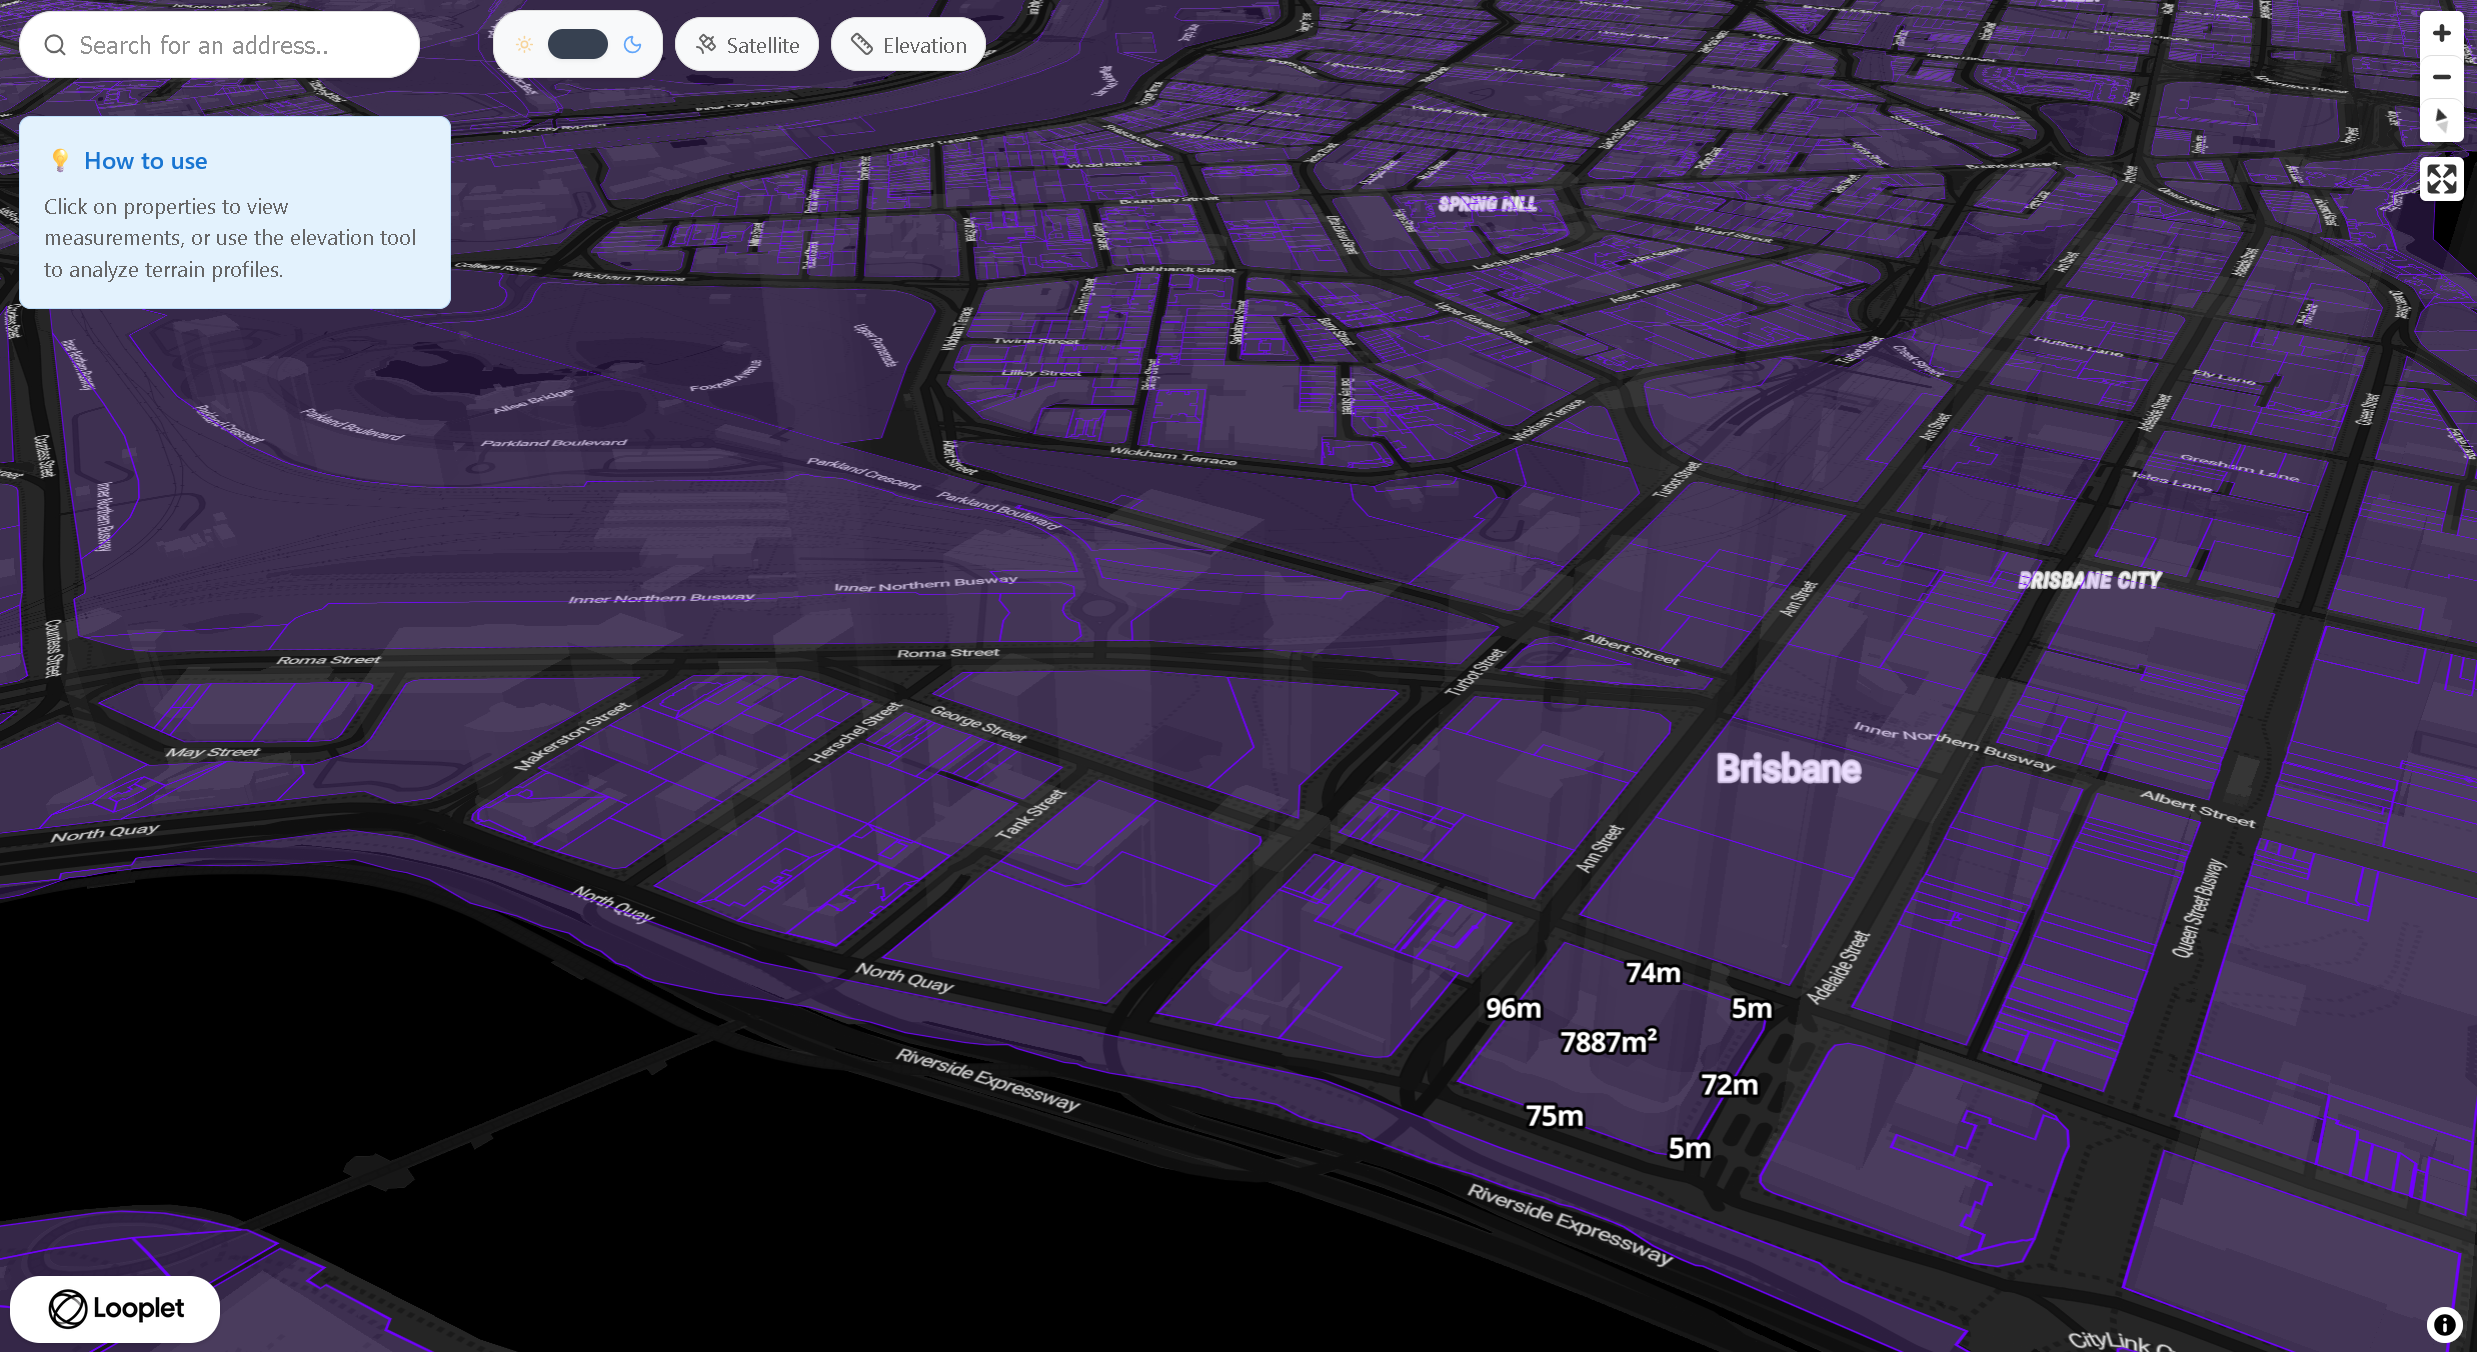
\includegraphics[scale=0.15]{figures/night_side_view.png}
    \caption{Night side view}
\end{figure}

Users can rotate the camera around to suit their needs.

\begin{figure}[H]
    \centering
    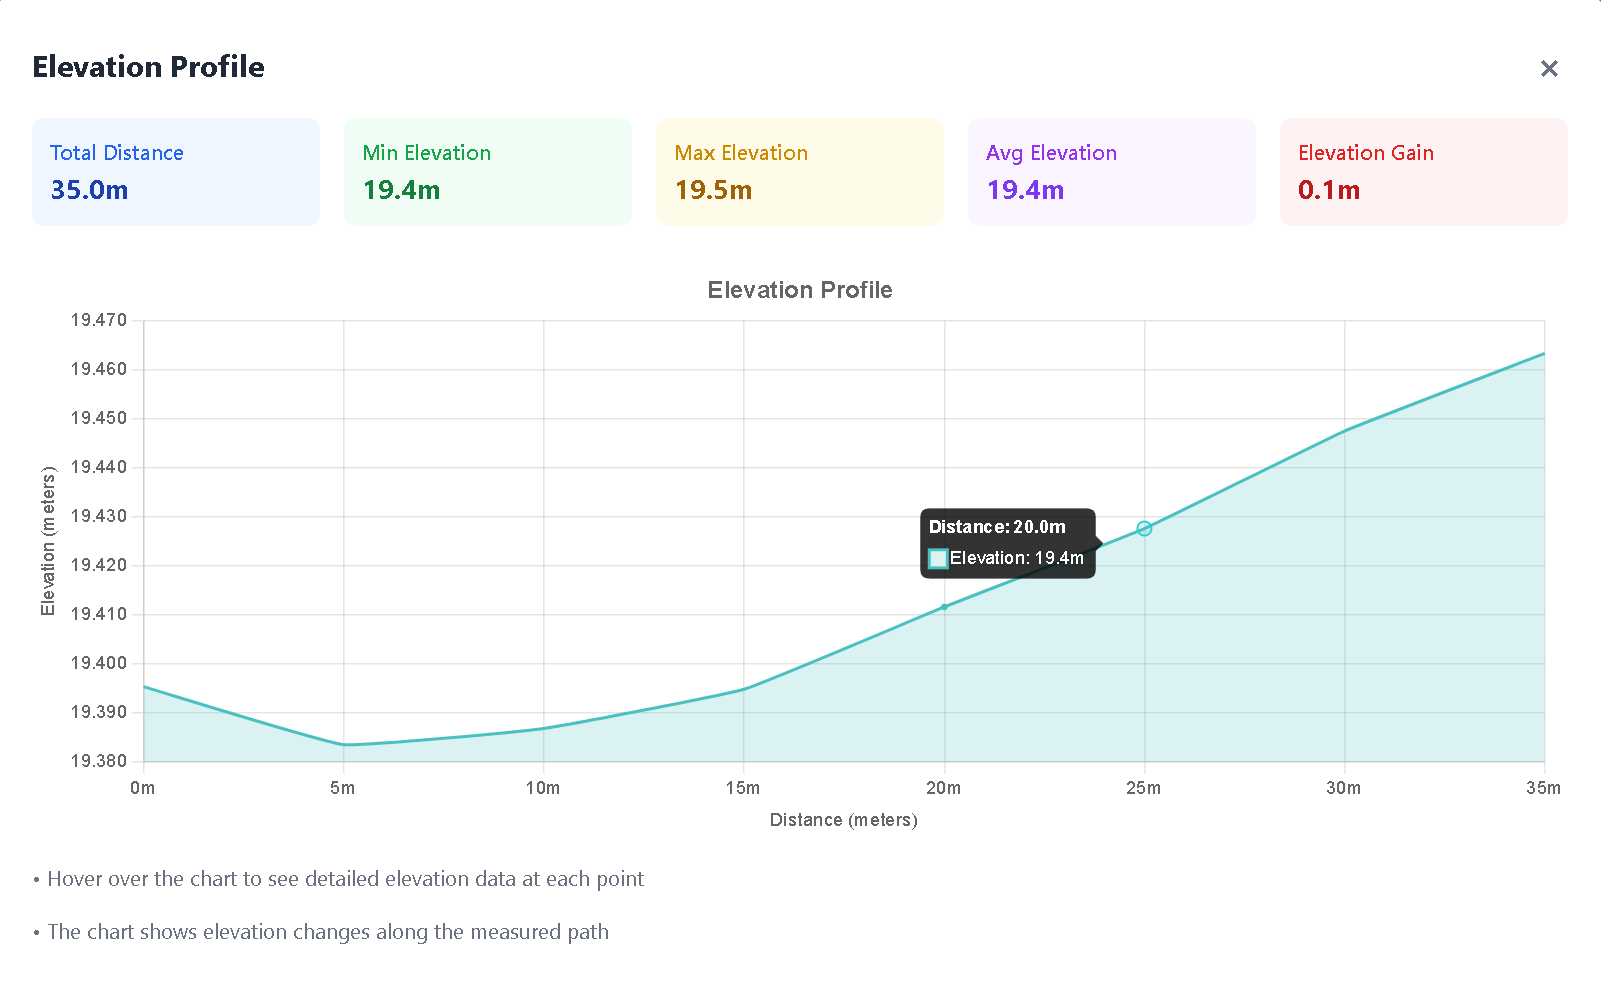
\includegraphics[scale=0.3]{figures/elevation_profile.png}
    \caption{Elevation profile}
\end{figure}

By selecting any two points on the map, the elevation profile can be obtained.

% TODO: Add figure of the Gemini stream API implementation
% \begin{figure}[H]
%     \centering
%     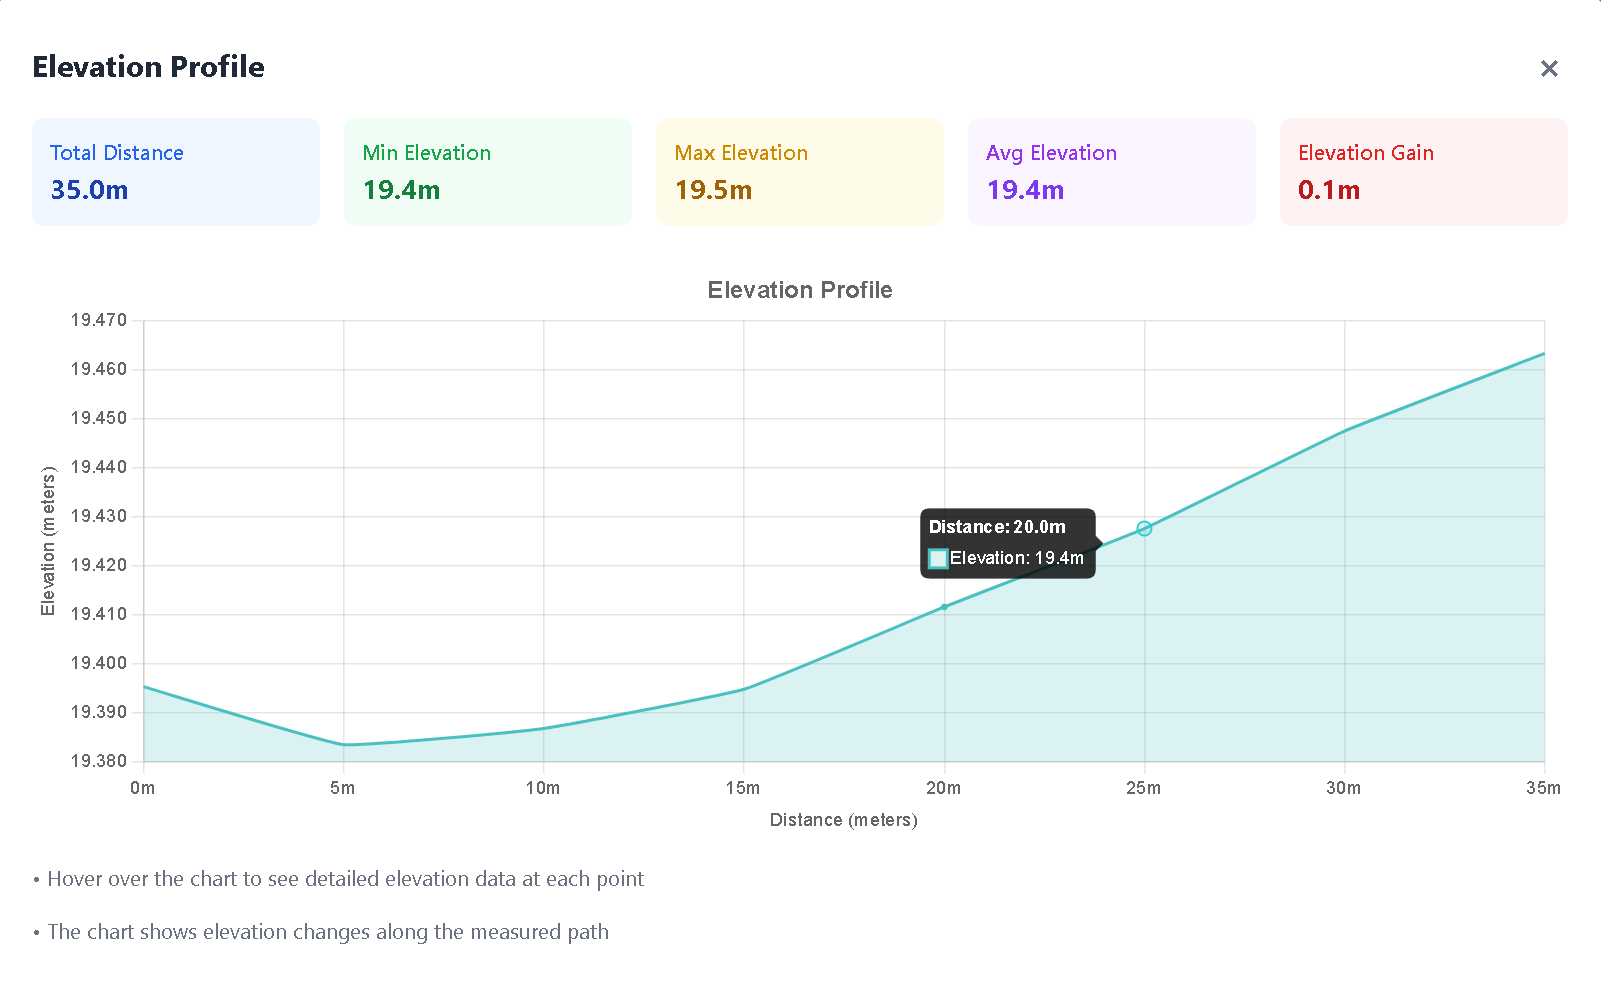
\includegraphics[scale=0.3]{figures/elevation_profile.png}
%     \caption{Gemini housing market prediction}
% \end{figure}